% !TEX encoding = UTF-8 Unicode
\documentclass[
11pt,
master, % тип документа
subf, % подключить и настроить пакет subfig для вложенной нумерации рисунков
href, % подключить и настроить пакет hyperref
colorlinks=true, % цветные гиперссылки
times, % шрифт Times как основной
%fixint=false % отключить прямые знаки интегралов
]{disser}
\usepackage[left=25mm, top=20mm, right=10mm, bottom=20mm]{geometry}
\usepackage[T2A]{fontenc}
\usepackage[utf8]{inputenc}
\usepackage[english,russian]{babel}
\usepackage{amsmath,amssymb,cmap} % cmap для кодировки шрифтов в pdf
\usepackage{pdfpages} % вставляем pdf файлы
\usepackage{indentfirst} % отделять первую строку раздела абзацным отступом
\usepackage{titletoc} % убираем отступ перед "Оглавление"
\usepackage{graphicx}
\usepackage{setspace}
\usepackage{verbatim} % для оформления кода
\usepackage{pdfsync} % установка соответствия документ - код
\graphicspath{{./Img/}}

\setlength\parindent{5ex} % абзацный отступ равный пяти строчным буквам основного шрифта
\pagestyle{plain} % включаем нумерацию
\setcounter{tocdepth}{2} % включать подсекции в оглавление
\linespread{1.3} % полуторный интервал


% Номера страниц снизу и по центру
\pagestyle{footcenter}
\chapterpagestyle{footcenter}

\begin{document}

\pagestyle{empty}
\begin{center}

\noindent  Федеральное государственное бюджетное образовательное учреждение\\
высшего профессионального образования\\

Московский государственный технический университет им. Н.Э. Баумана \\
Факультет <<Фундаментальные науки>>\bigskip\\

\vfill

Лабораторная работа №7\\
по курсу «Вычислительная физика»\\
Тема: «Метод Монте Карло»\\
\textbf{Вариант 6}\\


\vfill
\vfill
\begin{flushright}
\begin{tabular}{ll}
Выполнили: & студенты группы ФН4-72Б     \\
           & Хижик А.И., Мистрюкова Л.А. \\
Проверил:  & доцент, к.физ.-мат.н.       \\
           & Хасаншин Р.Х.
\end{tabular}
\end{flushright}
\vfill
\begin{center}
Москва, $2019$
\end{center}

\end{center}
\pagebreak


\pagestyle{plain} % нумерация вкл.
\tableofcontents

\section{Теоретическая часть}
\subsection{Введение}
В математической физике часто встречаются задачи, сводящиеся к следующему интегралу:
\begin{equation}\label{eq1}
  \frac{1}{\pi^2}\int_{S}\int_{S}f(\rho) dPdQб
\end{equation}
где $S$ -- единичный шар, $P$, $Q \in S$, $\rho = |P-Q|$ --
Предположим, что $P$ и $Q$ равномерно распределены в единичном шаре $S$. Тогда их плотности распределения равны:
$$p(P) = p(Q) = \frac{3}{4\pi}.$$

Рассмотрим сферическую систему координат $(r, \varphi, \mu)$, $\mu = \cos(\theta)$, $dP = -r^2 drd\varphi d\mu$. Возьмём точку $P$ на оси $0z$.
\begin{figure}[h]
  \centering
  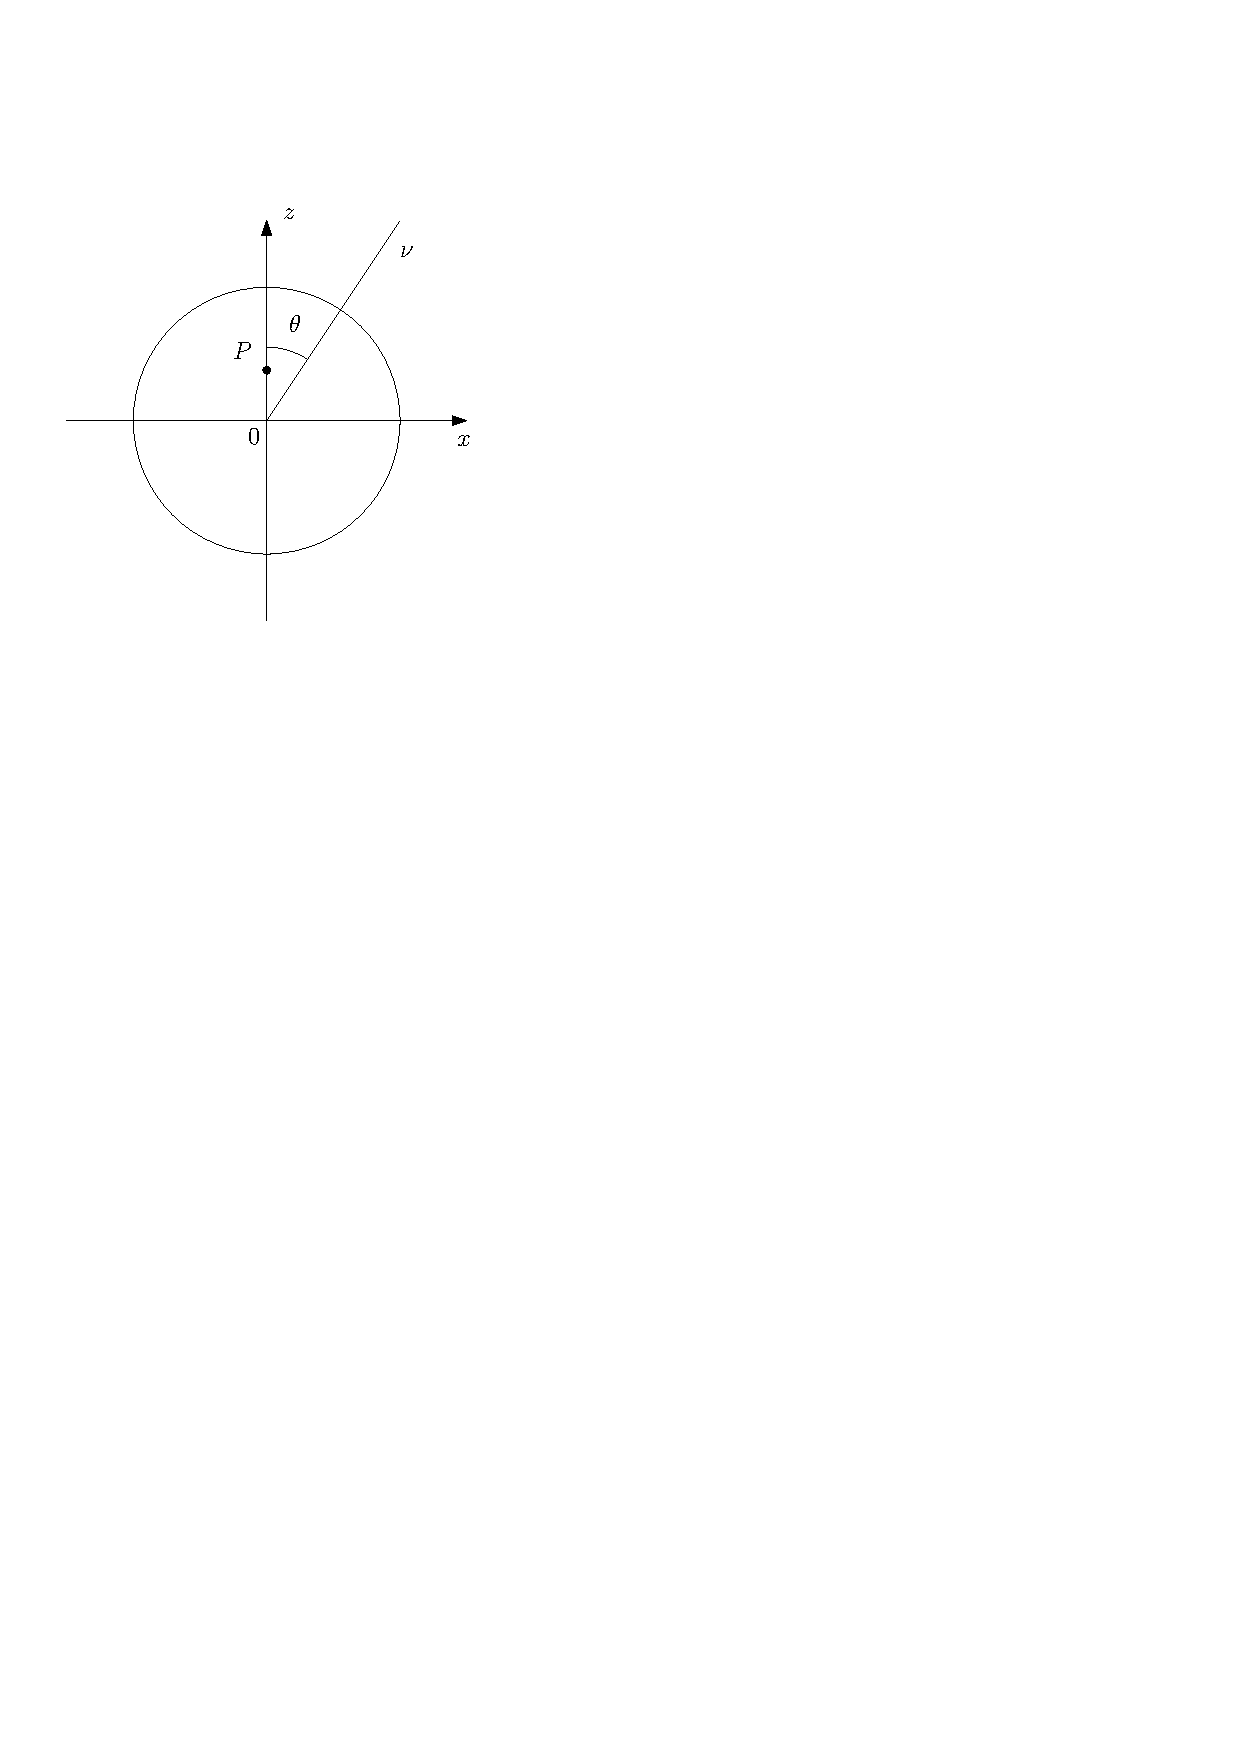
\includegraphics[width=0.4\linewidth]{ris1}
  \caption{}\label{ris:1}
\end{figure}

$$3\int_{0}^{r_P} r^2 dr = \gamma_{i+1}.$$
Не теряя общности возьмём точку $Q$ на плоскости $0xz$, т.е. при $\varphi = 0$. Для этого разыграем точку $Q$ на произвольном направлении $\nu$. Таким образом точка $Q$ выбирается по следующим законам:
$$\int_{-1}^{\mu_Q} \frac{d\mu}{2} = \gamma_{i+2},$$
$$3\int_{0}^{r_Q} r^2 dr = \gamma_{i+3}.$$

Следовательно, $r_P = \sqrt[3]{\gamma_{i+1}}$, $\mu_Q = 2\gamma_{i+2} - 1$, $r_Q = \sqrt[3]{\gamma_{i+3}}$ и $\rho = \sqrt{r_P^2 + r_Q^2 - 2r_P r_Q \mu_Q}$,\;$i = \overline{0,N-1}$.
Для вычисления интеграла (\ref{eq1}) определим среднее значение подынтегральной функции.
$$M\left[\frac{f(\rho)}{p(P)p(Q)}\right] = \int_{S}\int_{S}\frac{f(\rho)}{p(P)p(Q)} p(P)p(Q)dPdQ = \pi^2 I \Rightarrow I = \frac{1}{\pi^2} M\left[\frac{f(\rho)}{p(P)p(Q)}\right] = \frac{16}{9}M[f(\rho)].$$
При достаточно больших $N$: $M[f(\rho)] = \frac{1}{N}\sum_{i=0}^{N-1} f(\rho_i)$,
\begin{equation}\label{eq2}
  I \approx \overline{I} = \frac{16}{9N}\sum_{i=0}^{N-1} f(\rho_i)
\end{equation}

\subsubsection{Вычисление интегралов с особенностями}
Особенности могут быть двух видов: особенность подынтегральной функции на ограниченной области и бесконечная область интегрирования.

В первом случае используют существенную выборку, а именно, подбирают плотность вероятности содержащую ту же особенность что и подынтегральная функция.

Во втором случае:
\begin{enumerate}
  \item Если возможно, то с помощью преобразования координат перейти к первому случаю;
  \item Отбросить часть интеграла от достаточно удалённой области;
  \item Использовать существенную выборку, когда плотность вероятности достаточно быстро убывает с ростом границы области интегрирования.
\end{enumerate}

Предположим, что подынтегральная функция интеграла (\ref{eq1}) содержит особенность $\sim \rho^{-2}$. Подберем плотность вероятности пропорциональную $\rho^{-2}$.

Пусть независимые случайные точки $P$ и $Q$ распределены следующим образом: точка $P$ равномерно распределена в шаре $p(P) = \frac{3}{4\pi}$, точку $Q$ ищем на плоскости $0xz$, $p(Q) \sim \rho^{-2}$. Для этого рассмотрим сферическую систему координат $(r,\varphi,\mu)$,
\begin{figure}[h]
  \centering
  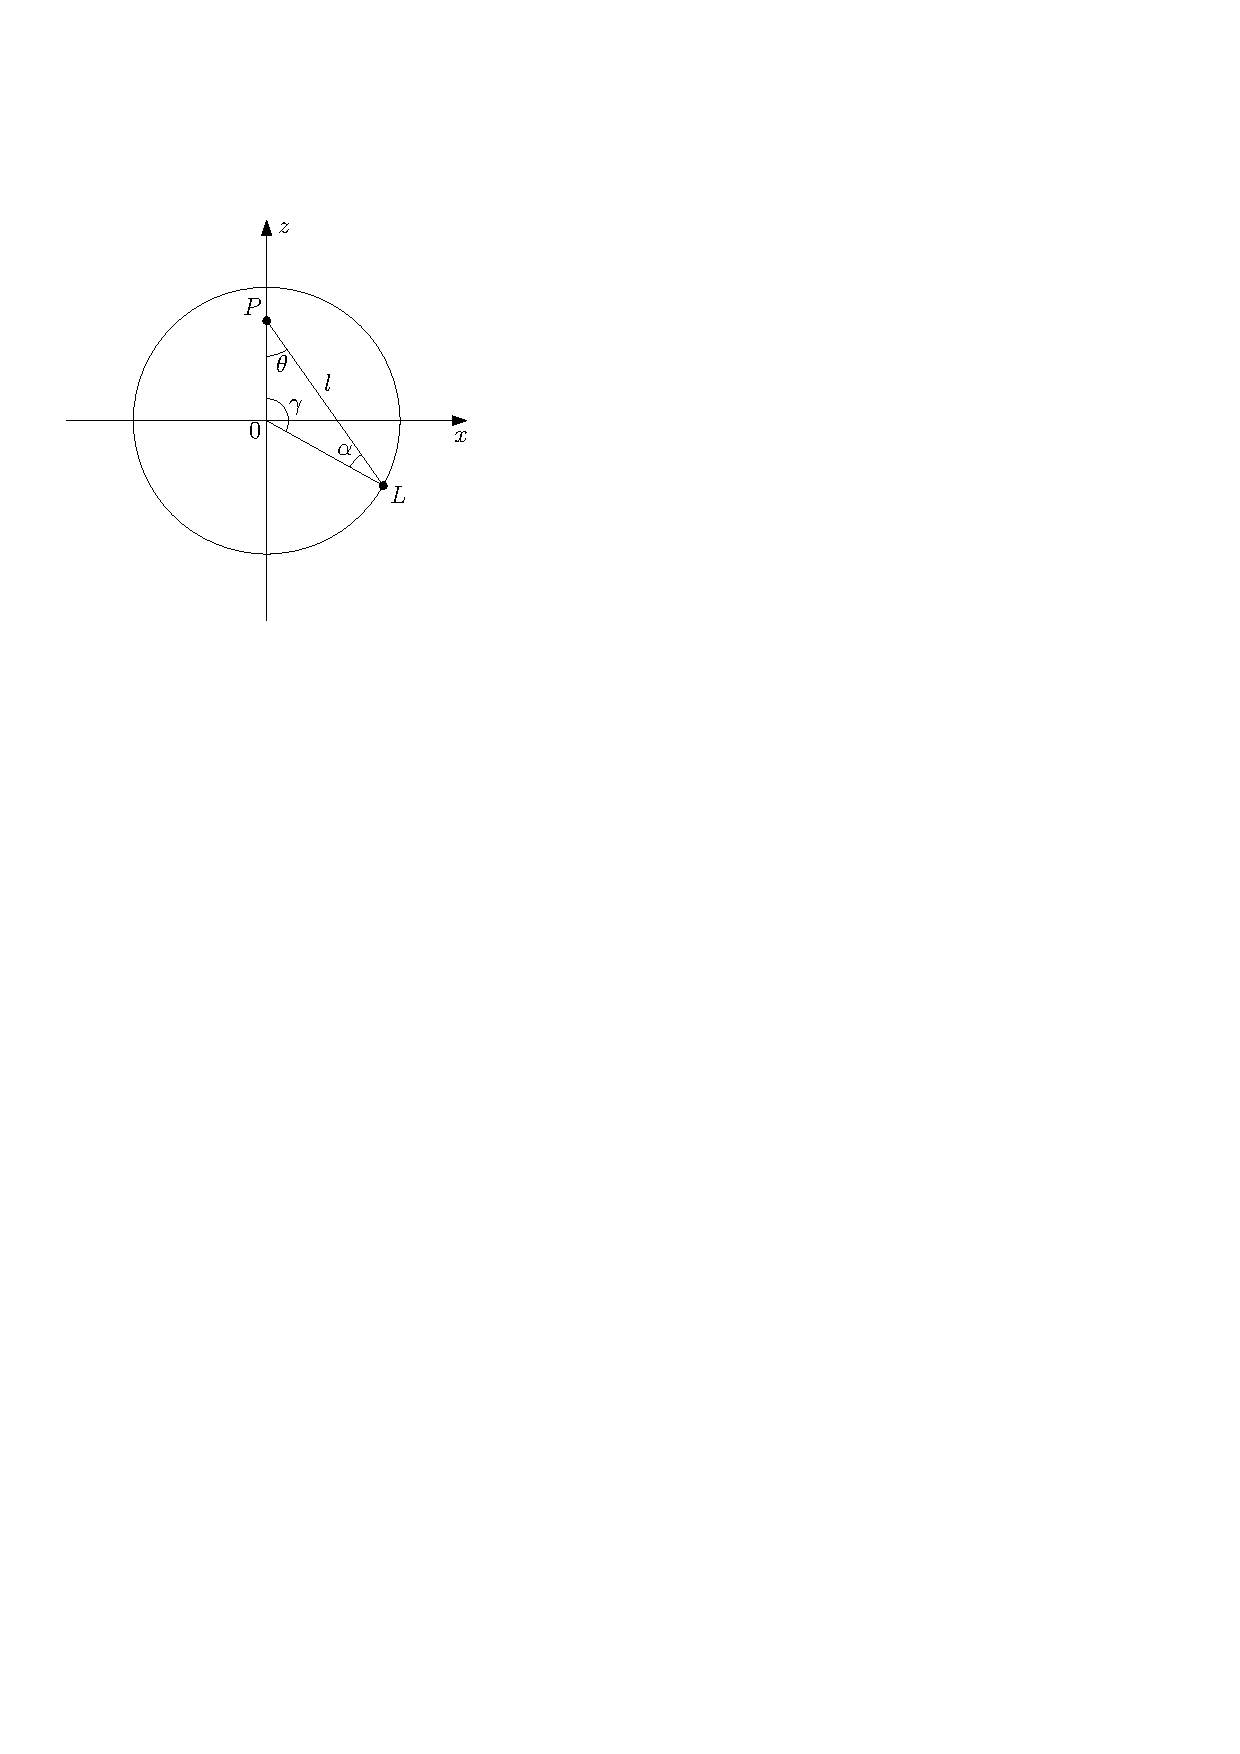
\includegraphics[width=0.4\linewidth]{ris2}
  \caption{}\label{ris:2}
\end{figure}

$$\mu = \cos(\theta),$$
$$\int_{-1}^{\mu_Q} \frac{d\mu}{2} = \gamma_{i+2},$$
$$p(Q) = \frac{1}{4\pi l \rho^2}.$$
Используя теорему синусов, получаем
$$l = r_P \mu_Q + \sqrt{1 - r_P^2(1-\mu_Q^2)}.$$
Предыдущие манипуляции позволяют получит следующие расчётные формулы:
$$r_P = \sqrt[3]{\gamma_{i+1}},\;\; \mu_Q = 2\gamma_i - 1,\;\; l = r_P \mu_Q + \sqrt{1 - r_P^2(1-\mu_Q^2)},$$
$$M\left[\frac{f(\rho)}{p(P)p(Q)}\right] = \frac{16}{3} M[f(\rho)\rho^2l],$$
\begin{equation}\label{eq3}
  I \approx \tilde{I} = \frac{16}{3N}\sum_{i=0}^{N-1} f(\rho_i)\rho_i^2 l_i.
\end{equation}

\subsection{Методы понижения дисперсии}
Все методы и приемы рассмотренные для вычисления одномерных интегралов без затруднений переносятся на многомерный случай.
\subsubsection{Интегрирование по части переменных}
Пусть $\int_{V_P}\int_{V_Q} f(P,Q) p(P,Q) dPdQ$, где точки $P \in V_P$, $Q\in V_Q$, $p(P,Q)$ -- плотность
распределения.

Пусть $\tilde{p}(P) = \int_{V_Q} p(P,Q)dQ \rightarrow \tilde{f}(P)\tilde{p}(P) = \int_{V_Q} f(P,Q)p(P,Q)dQ$. Очевидно, что\\
$I = \int_{V_P} \tilde{f}(P)\tilde{p}(P)dP$.

\textbf{Утверждение}: $D[\tilde{f}] \leq D[f]$.

\textbf{Доказательство}: пусть $u(x)$, $v(x) \in \mathbb{L}_2(G)$, используем неравенство Коши-Буняковского:\\ $|\langle u, v \rangle| \leq \|u\|\|v\|$.
$$\left(\int_{G} u(x)v(x)dx\right)^2 \leq \int_{G} u^2(x)dx \int_{G} v^2(x)dx$$

Пусть $p(P) \geq 0$ в $G$ и $u(P), v(P) \in \mathbb{L}_2(G;p)$. Тогда
$$\left(\int_{G} u(P)v(P)p(P)dP\right)^2 \leq \int_{G} u^2(P)p(P)dP \int_{G} v^2(P)p(P)dP,$$,
$$\forall z \in \mathbb{R}:\;\; 0\leq \int_{G} [zu(P) + v(P)]^2p(P)dP \Longleftrightarrow 0\leq az^2 + 2bz + c \Rightarrow b^2 - ac \leq 0,$$
$$\tilde{f}^2(P) \tilde{p}^2(P) = \left[\int_{V_Q} f(P,Q) p(P,Q) dQ\right]^2 \leq \int_{V_Q} f^2(P,Q)p(P,Q)dQ\int_{V_Q} p(P,Q)dQ,$$
$$\tilde{f}^2(P)\tilde{p}^2(P) \leq \tilde{p}(P)\int_{V_Q} f^2(P,Q)p(P,Q)dQ.$$
Проинтегрируем полученное неравенство по $V_P$:
$$D[\tilde{f}] \leq D[f].$$

\subsubsection{Выборка по группам}
$I = \int_{G} f(P)p(P)dP$. Пусть $G = \sum_{i=1}^{m} G_i \rightarrow I_i = \int_{G_i}f(P)p(P)dP$, $p_i = \int_{G_i}p(P)dP$. Введем в области $G_i$ случайную величину $\xi^{(i)}$ с плотностью вероятности $\frac{p(P)}{p_i}$. Возьмём $N_i$ значений случайно величины $\xi^{(i)}:\left\{\xi_k^{(i)}\right\}$. Тогда $I_i \approx \frac{p_i}{N_i} \sum_{k=1}^{N_i} f\left(\xi_k^{(i)}\right)$,
$$I \approx \sum_{i=1}^{m} \frac{p_i}{N_i} \sum_{k=1}^{N_i}f\left(\xi_k^{(i)}\right).$$

Этот метод по своей идее близок к методу существенной выборки: здесь также предлагается выбирать больше точек в более «существенных» областях, однако выбор регулируется не специально подобранной плотностью распределения, а указанием количества точек в различных областях интегрирования.
\newpage
\section{Постановка задачи}
\begin{itemize}
\item Вычислить ММК интеграл $\displaystyle I_m = \frac{1}{\pi^2}\int_S\int_S \frac{dP dQ}{\rho^m}$ при $m=1$ и $m=2$, где $S$ -- единичный трёхмерный шар, $P$, $Q\in S$, $\rho = |P-Q|$, используя оценки $\displaystyle\overline{I} = \frac{16}{9N}\sum_{i=1}^{N}f(\rho_i)$ и $\displaystyle\tilde{I} = \frac{16}{3N}\sum_{i=1}^{N}f(\rho_i)\rho_i^2 l_i$. Сравнить полученные значения с точными.
\end{itemize}

\newpage
\section{Программа}

{\footnotesize
\begin{verbatim}
#include <iostream>
using namespace std;
#include <random>
#include <cmath>

double N = 1e6;
double fun1(double dis, double m);

int main()
{
    mt19937 gen{random_device()()};
    uniform_real_distribution <double> dist(0.0, 1.0);
    double r1, mu2, r2, dis1, dis2, l;
    double sum11 = 0, sum12 = 0, sum21 = 0, sum22 = 0;
    double Integral1(2.133), Integral2(4.000);

    for (int i = 0; i < N-1; i++) {
        r1 = pow(dist(gen), 1. / 3);
        mu2 = 2 * dist(gen) - 1;
        r2 = pow(dist(gen), 1. / 3);
        dis1 = sqrt(r1*r1 + r2*r2 - 2*r1*r2*mu2);
        l = r1*mu2 + sqrt(1 - r1*r1*(1 - mu2*mu2));
        dis2 = l*dist(gen);
        sum11 += fun1(dis1, 1.);
        sum12 += fun1(dis2, 1.) * dis2*dis2 * l;
        sum21 += fun1(dis1, 2.);
        sum22 += fun1(dis2, 2.) * dis2*dis2 * l;
    }

    cout << "Number of steps: " << N << endl;

    double Integral11 = 16 * sum11 / (9*N);
    double AbsError11 = abs(Integral11 - Integral1);
    double Disp11 = N / 9 * pow(AbsError11, 2);

    cout << "m = 1\n" << "I1 = " << Integral11 << endl;
    cout << "AbsError = " << AbsError11 << endl;
    cout << "Dispersion = " << Disp11 << "\n\n";

    double Integral12 = 16 * sum12 / (3*N);
    double AbsError12 = abs(Integral12 - Integral1);
    double Disp12 = N / 9 * pow(AbsError12, 2);

    cout << "I2 = " << Integral12 << endl;
    cout << "AbsError = " << AbsError12 << endl;
    cout << "Dispersion = " << Disp12 << "\n\n";

    double Integral21 = 16 * sum21 / (9*N);
    double AbsError21 = abs(Integral21 - Integral2);
    double Disp21 = N / 9 * pow(AbsError21, 2);

    cout << "m = 2\n" << "I1: " << Integral21 << endl;
    cout << "AbsError = " << AbsError21 << endl;
    cout << "Dispersion = " << Disp21 << "\n\n";

    double Integral22 = 16 * sum22 / (3*N);
    double AbsError22 = abs(Integral22 - Integral2);
    double Disp22 = N / 9 * pow(AbsError22, 2);

    cout << "I2: " << Integral22 << endl;
    cout << "AbsError = " << AbsError22 << endl;
    cout << "Dispersion = " << Disp22 << "\n\n";
    return 0;
}
double fun1(double dis, double m)
{
    return 1 / pow(dis, m);
}
\end{verbatim}
}

\newpage
\section{Результаты вычислений}
\subsubsection{Вычисленные значения интеграла $\displaystyle I_m = \frac{1}{\pi^2}\int_S\int_S \frac{dP dQ}{\rho^m}$ для a) $m=1$ и b) $m=2$ при использовании оценок $\displaystyle\overline{I}= I1 = \frac{16}{9N}\sum_{i=1}^{N}f(\rho_i)$, $\displaystyle\tilde{I} = I2 = \frac{16}{3N}\sum_{i=1}^{N}f(\rho_i)\rho_i^2 l_i$ для различных статистик $N$}
\begin{figure}[h]
\begin{minipage}[h]{0.48\linewidth}
\center{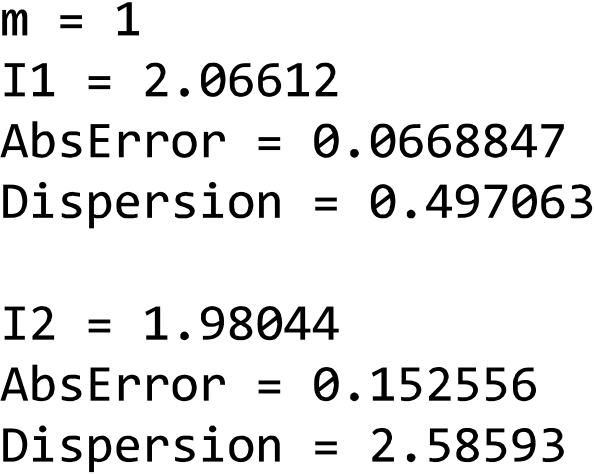
\includegraphics[width=1\linewidth]{res7}} a) \\
\end{minipage}
\hfill
\begin{minipage}[h]{0.48\linewidth}
\center{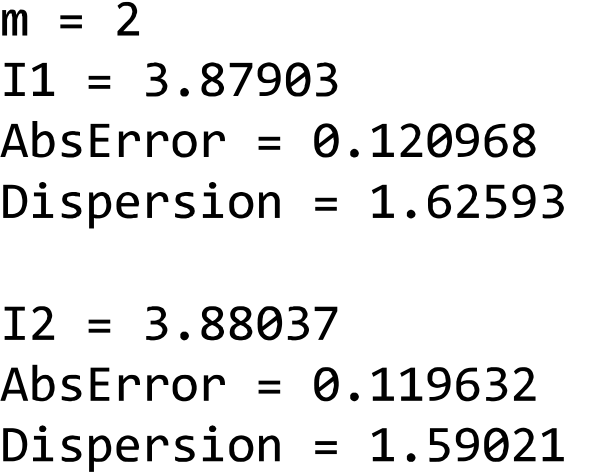
\includegraphics[width=1\linewidth]{res8}} b) \\
\end{minipage}
\caption{$N = 10^3$}
\label{ris:3}
\end{figure}

\begin{figure}[h]
\begin{minipage}[h]{0.48\linewidth}
\center{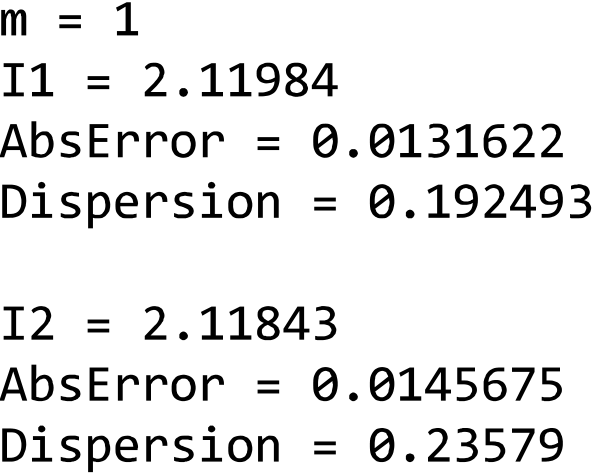
\includegraphics[width=1\linewidth]{res5}} a) \\
\end{minipage}
\hfill
\begin{minipage}[h]{0.48\linewidth}
\center{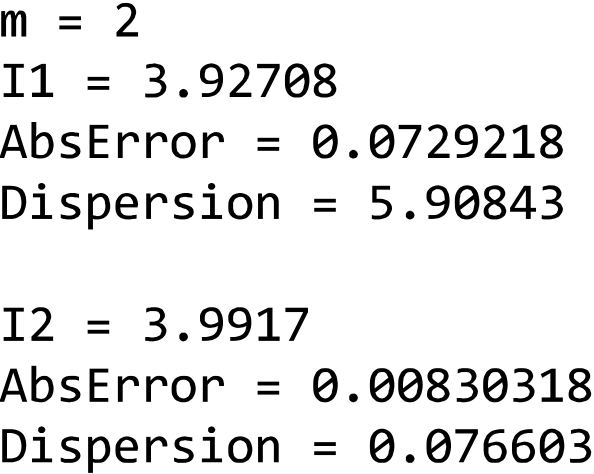
\includegraphics[width=1\linewidth]{res6}} b) \\
\end{minipage}
\caption{$N = 10^4$}
\label{ris:4}
\end{figure}

\begin{figure}[h]
\begin{minipage}[h]{0.48\linewidth}
\center{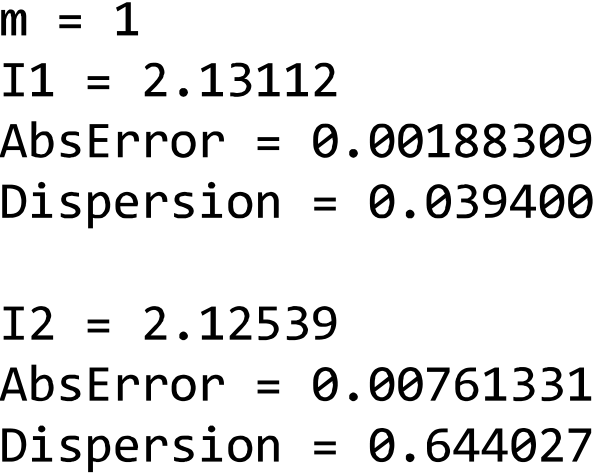
\includegraphics[width=1\linewidth]{res3}} a) \\
\end{minipage}
\hfill
\begin{minipage}[h]{0.48\linewidth}
\center{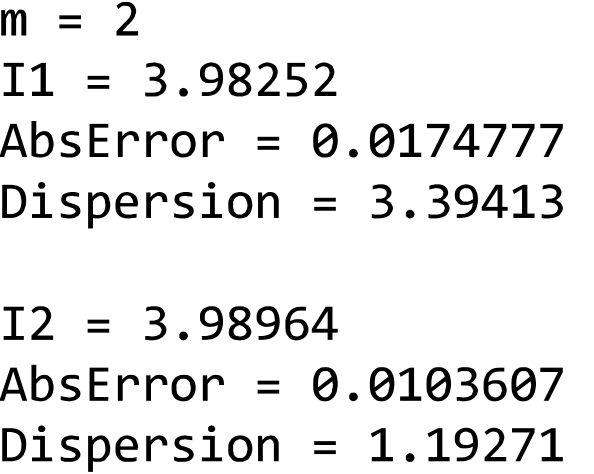
\includegraphics[width=1\linewidth]{res4}} b) \\
\end{minipage}
\caption{$N = 10^5$}
\label{ris:5}
\end{figure}

\begin{figure}[h]
\begin{minipage}[h]{0.48\linewidth}
\center{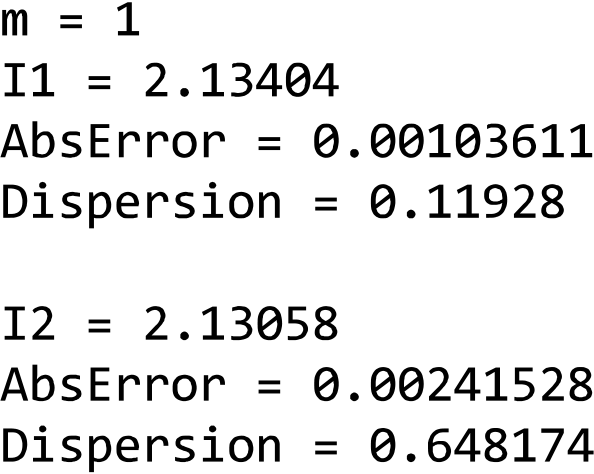
\includegraphics[width=1\linewidth]{res1}} a) \\
\end{minipage}
\hfill
\begin{minipage}[h]{0.48\linewidth}
\center{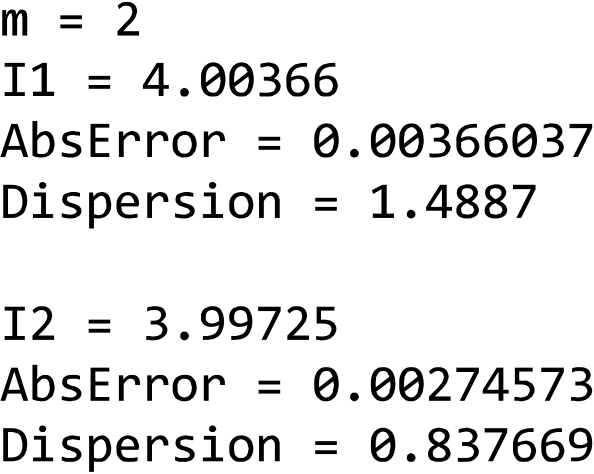
\includegraphics[width=1\linewidth]{res2}} b) \\
\end{minipage}
\caption{$N = 10^6$}
\label{ris:6}
\end{figure}

\section{Вывод}
Методом Монте-Карло был вычислен многомерный интеграл $\displaystyle I_m = \frac{1}{\pi^2}\int_S\int_S \frac{dP dQ}{\rho^m}$ при $m=1$ и $m=2$, используя оценки $\displaystyle\overline{I} = \frac{16}{9N}\sum_{i=1}^{N}f(\rho_i)$, $\displaystyle\tilde{I} = \frac{16}{3N}\sum_{i=1}^{N}f(\rho_i)\rho_i^2 l_i$ для статистики $N = 10^6$.

При вычислении интеграла $I_1$ наибольшую точность при одной и той же статистике позволяет достичь приближение $\displaystyle\overline{I}$, в свою очередь, оценка $\displaystyle\tilde{I}$ значительно точнее оценки $\displaystyle\overline{I}$ при вычислении интеграла $I_2$.

\end{document} 